\documentclass[border=3pt]{standalone}
% Preâmbulo compartilhado pelos diagramas TikZ da aula
\usepackage[T1]{fontenc}
\usepackage[utf8]{inputenc}
\usepackage{lmodern}
\usepackage{amsmath}
\usepackage{xcolor}
\usepackage{tikz}
\usetikzlibrary{arrows.meta,angles,quotes,decorations.pathmorphing,calc,
                positioning,shapes.geometric,backgrounds,fit}

% Paleta (mesma dos SVGs originais)
\definecolor{dblue}{HTML}{2A5B8C}
\definecolor{dorange}{HTML}{B3541E}
\definecolor{dgreen}{HTML}{4A7C59}
\definecolor{dred}{HTML}{9C4B4B}
\definecolor{dcream}{HTML}{F4F1EA}
\definecolor{dshade}{HTML}{DDD7C9}

% Estilos comuns (prefixo d... para não colidir com chaves internas do pgf)
\tikzset{
  >={Stealth[length=2mm]},
  dguide/.style={gray!55, dashed, line width=0.4pt},
  daxis/.style={gray!60, line width=0.7pt, ->},
  dbody/.style={fill=black!3, draw=black!80, line width=1pt},
  dacc/.style={draw=dblue, line width=1pt},
  dlbl/.style={black!55, font=\small},
  dsub/.style={black!45, font=\footnotesize},
  dstate/.style={circle, draw=black!80, fill=dcream, line width=1pt,
                 minimum size=17mm, font=\large, inner sep=1pt},
  dobs/.style={circle, draw=black!80, fill=dshade, line width=1pt,
               minimum size=14mm, font=\large, inner sep=1pt},
  dbox/.style={rounded corners=2pt, draw=black!80, fill=dcream, line width=1pt,
               align=center, inner sep=6pt},
  dtrans/.style={->, dblue, line width=1pt},
  dmeas/.style={->, dorange, line width=1pt},
}

\begin{document}
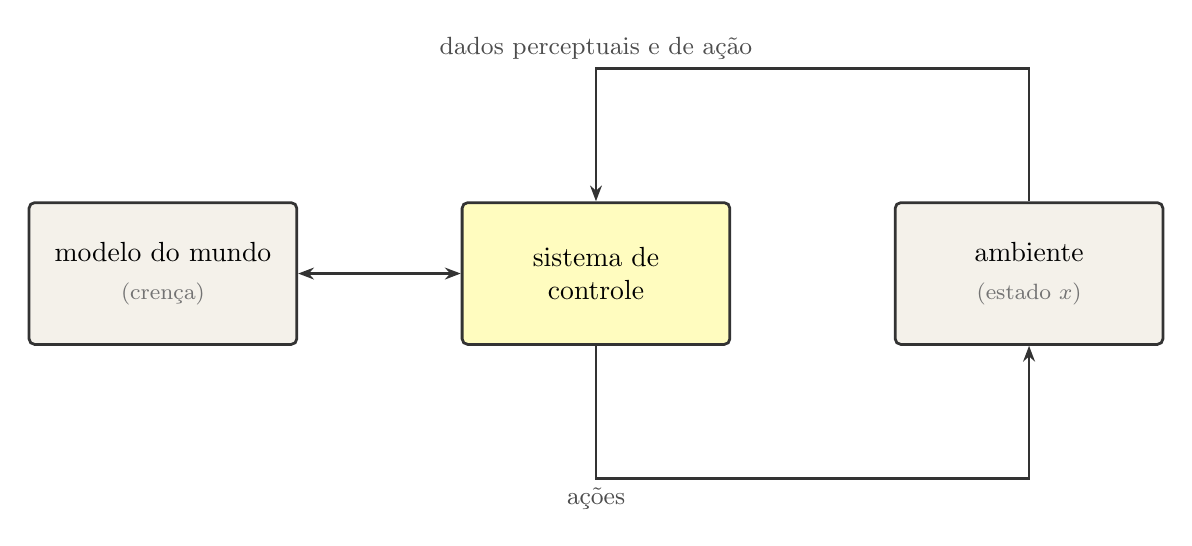
\begin{tikzpicture}[x=1cm,y=1cm]

  \node[dbox, minimum width=3.4cm, minimum height=1.8cm] (W) at (0,0)
       {modelo do mundo\\[2pt]\footnotesize\textcolor{black!55}{(crença)}};
  \node[dbox, fill=yellow!25, minimum width=3.4cm, minimum height=1.8cm] (C) at (5.5,0)
       {sistema de\\controle};
  \node[dbox, minimum width=3.4cm, minimum height=1.8cm] (E) at (11,0)
       {ambiente\\[2pt]\footnotesize\textcolor{black!55}{(estado $x$)}};

  % troca bidirecional modelo <-> controle
  \draw[<->, black!80, line width=1pt] (W) -- (C);

  % dados perceptuais/ação: ambiente -> controle (por cima)
  \draw[->, black!80, line width=1pt] (E.north) |- (5.5,2.6) -| (C.north);
  \node[black!70, font=\small, above] at (5.5,2.6) {dados perceptuais e de ação};

  % ações: controle -> ambiente (por baixo)
  \draw[->, black!80, line width=1pt] (C.south) |- (5.5,-2.6) -| (E.south);
  \node[black!70, font=\small, below] at (5.5,-2.6) {ações};

\end{tikzpicture}
\end{document}
